\chapter{Исследовательский раздел}

В данном разделе приведено исследование влияния стратегий индексирования на время выполнения процедуры \texttt{notify\_subscribers\_about\_new\_video}.
Измерения выполнены для разных масштабов данных и долей подписчиков целевого канала, чтобы понять, какие индексы дают наибольший эффект при росте нагрузки.


\section*{Технические характеристики ЭВМ}
Замеры проводились на устройстве со следующими характеристиками:
\begin{itemize}
    \item операционная система --- Microsoft Windows 11 Pro (64-разрядная);
    \item процессор --- AMD Ryzen 5 3600X, 6 физических ядер, 12 логических ядер, 3.79 ГГц;
    \item оперативная память --- 16 Гбайт.
\end{itemize}


\section{Проведение исследования}
Для каждого набора параметров база данных пересоздавалась и заполнялась данными.
Количество пользователей/подписок варьировалось в диапазоне от 10\,000 до 1\,000\,000.
Для тестового канала рассматривались доли подписчиков: 0.1\%, 1\%, 5\% и 10\%.

Измерения проводились по среднему времени выполнения хранимой процедуры за 20 повторов после 5 прогревочных запусков.
Между повторениями счётчики сбрасывались, а статистика обновлялась командой \texttt{ANALYZE}.
Для сравнения использовались следующие стратегии b-tree индексации:
\begin{enumerate}
    \item без индексов;
    \item индекс по \texttt{subscriptions(channel\_id)};
    \item индекс по \texttt{subscriptions(channel\_id, user\_id)};
    \item индекс по \texttt{users(notifications\_enabled, id)};
    \item частичный индекс по \texttt{users(id)} с условием \texttt{notifications\_enabled = true};
    \item комбинация индексов 2 и 3.
\end{enumerate}

Для наглядности приведены относительные гистограммы, где для каждого размера данных время нормировано по максимальному значению (0..1).

Относительные результаты для доли подписчиков 0.1\% представлены на рисунке~\ref{fig:benchmark-relative-0-001}.

\begin{figure}[H]
    \centering
    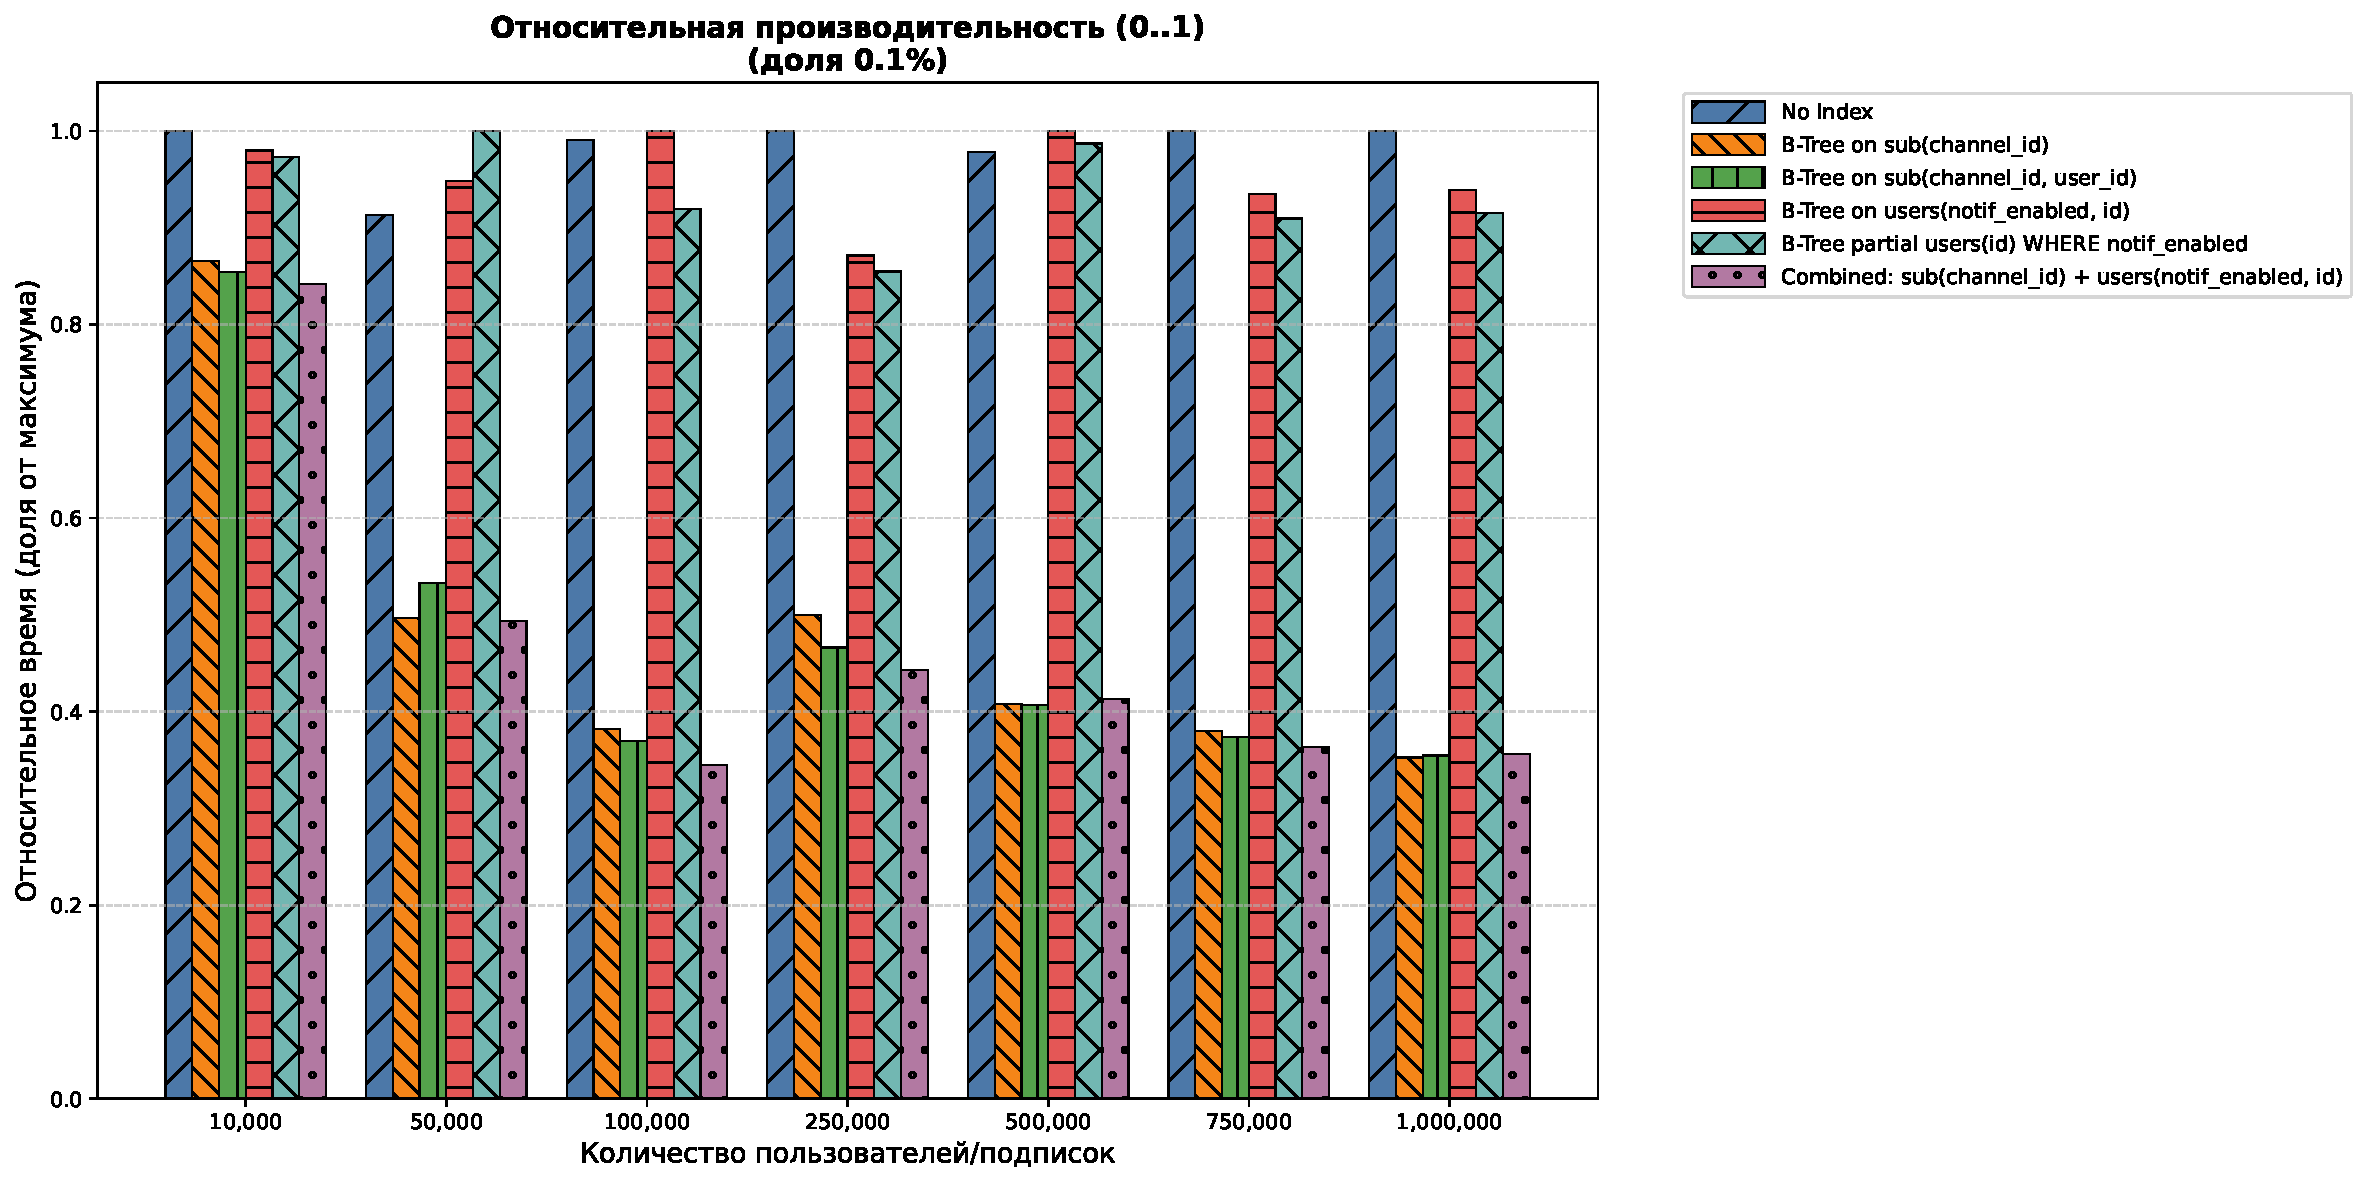
\includegraphics[width=1\linewidth]{images/benchmark_relative_0_001}
    \caption{Относительное время выполнения при доле подписчиков 0.1\%}
    \label{fig:benchmark-relative-0-001}
\end{figure}

Для доли 1\% результаты приведены на рисунке~\ref{fig:benchmark-relative-0-01}.

\begin{figure}[H]
    \centering
    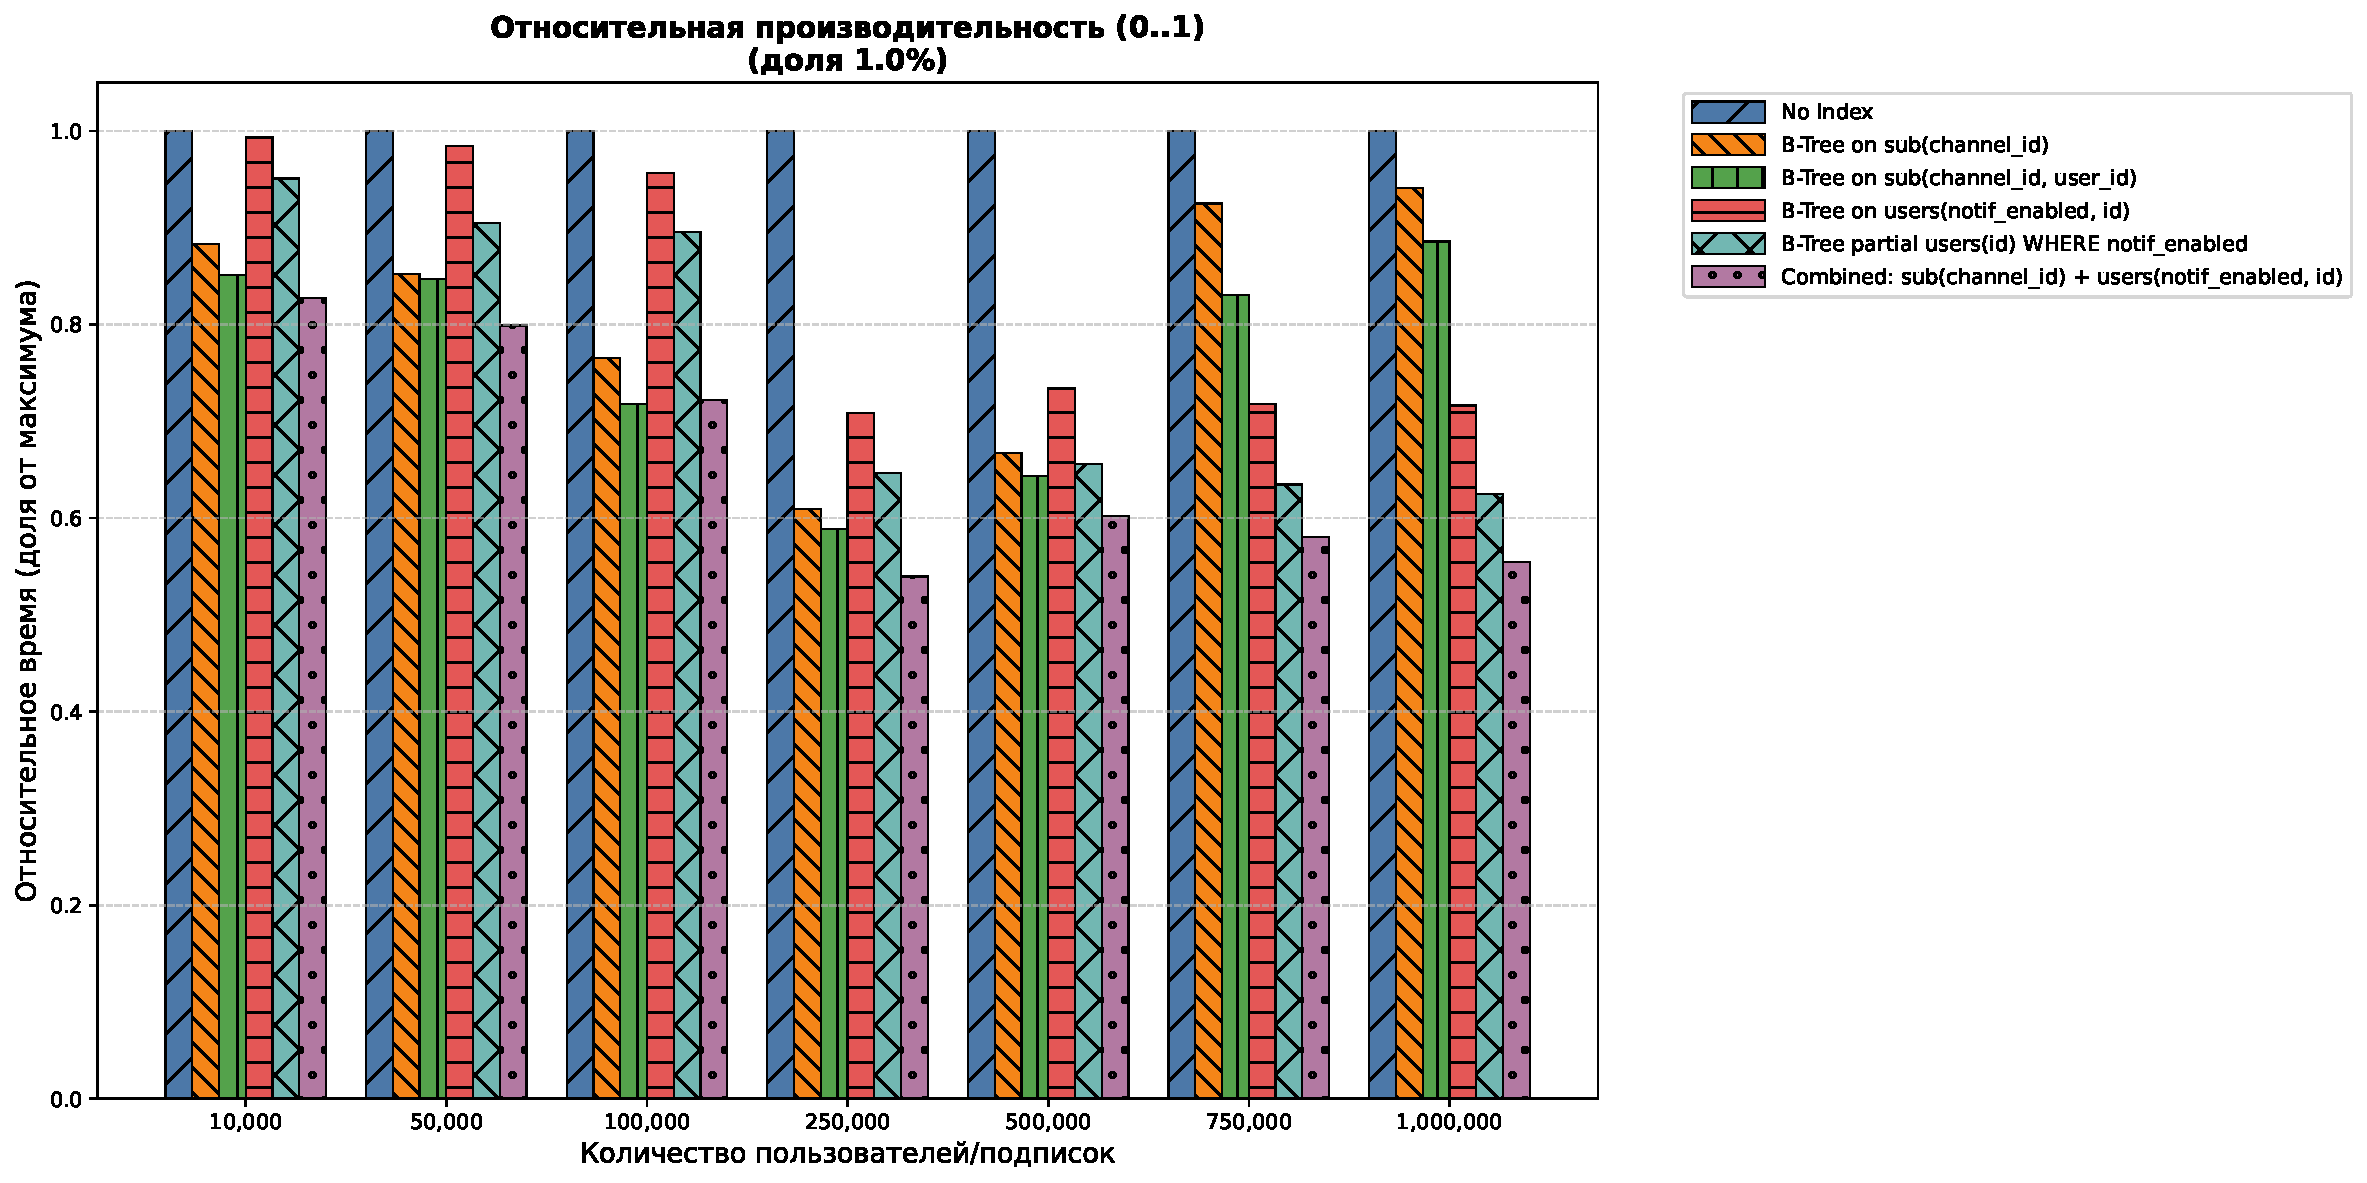
\includegraphics[width=1\linewidth]{images/benchmark_relative_0_01}
    \caption{Относительное время выполнения при доле подписчиков 1\%}
    \label{fig:benchmark-relative-0-01}
\end{figure}

Для доли 5\% результаты приведены на рисунке~\ref{fig:benchmark-relative-0-05}.

\begin{figure}[H]
    \centering
    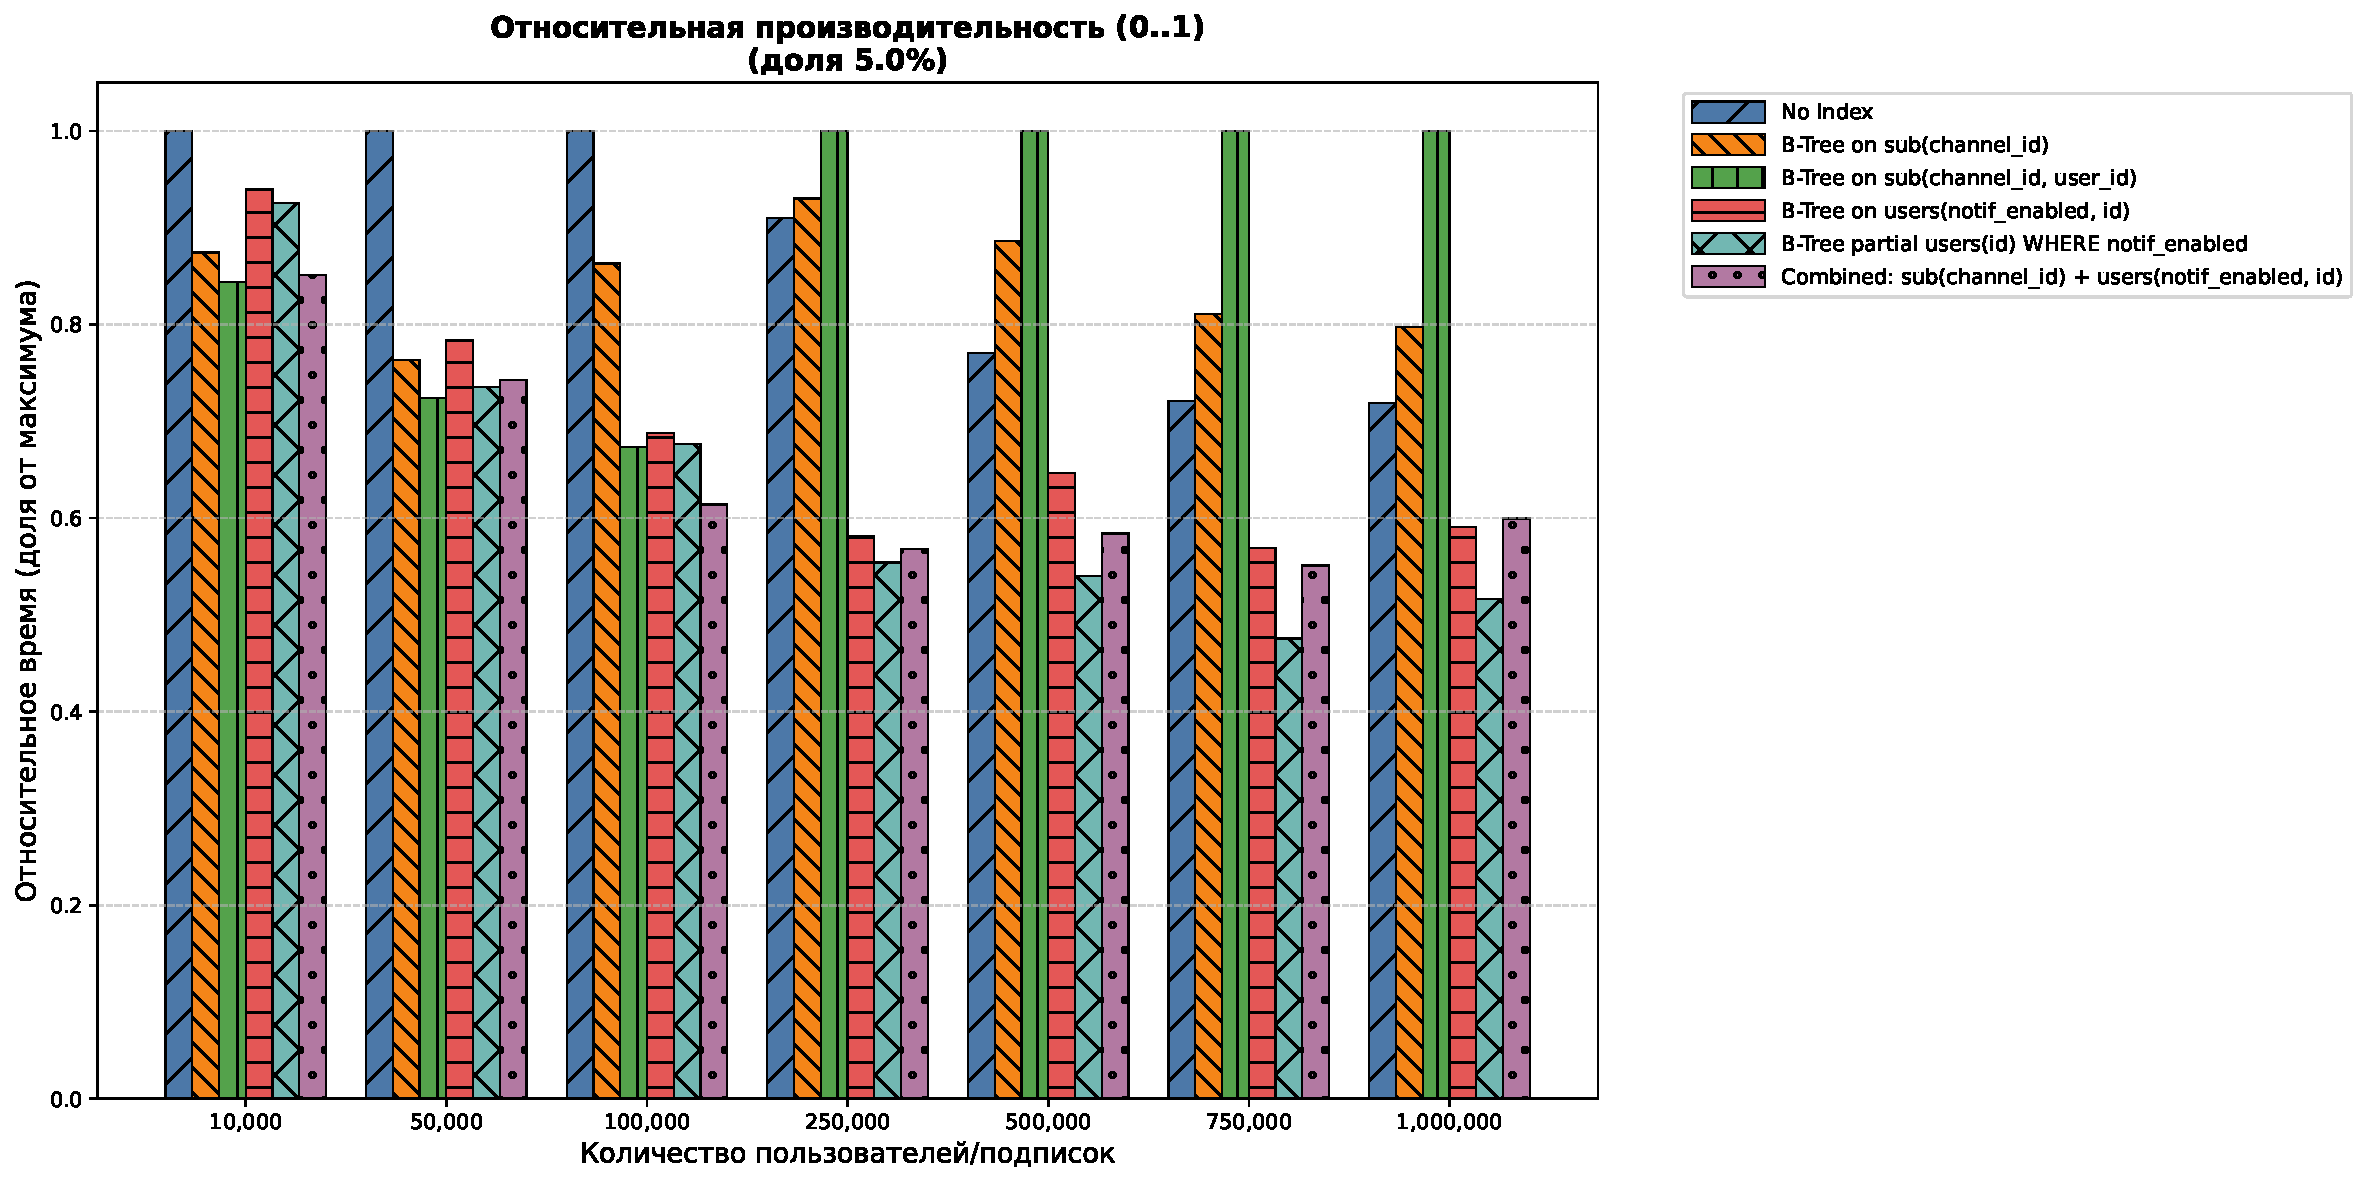
\includegraphics[width=1\linewidth]{images/benchmark_relative_0_05}
    \caption{Относительное время выполнения при доле подписчиков 5\%}
    \label{fig:benchmark-relative-0-05}
\end{figure}

Для доли 10\% результаты представлены на рисунке~\ref{fig:benchmark-relative-0-1}.

\begin{figure}[H]
    \centering
    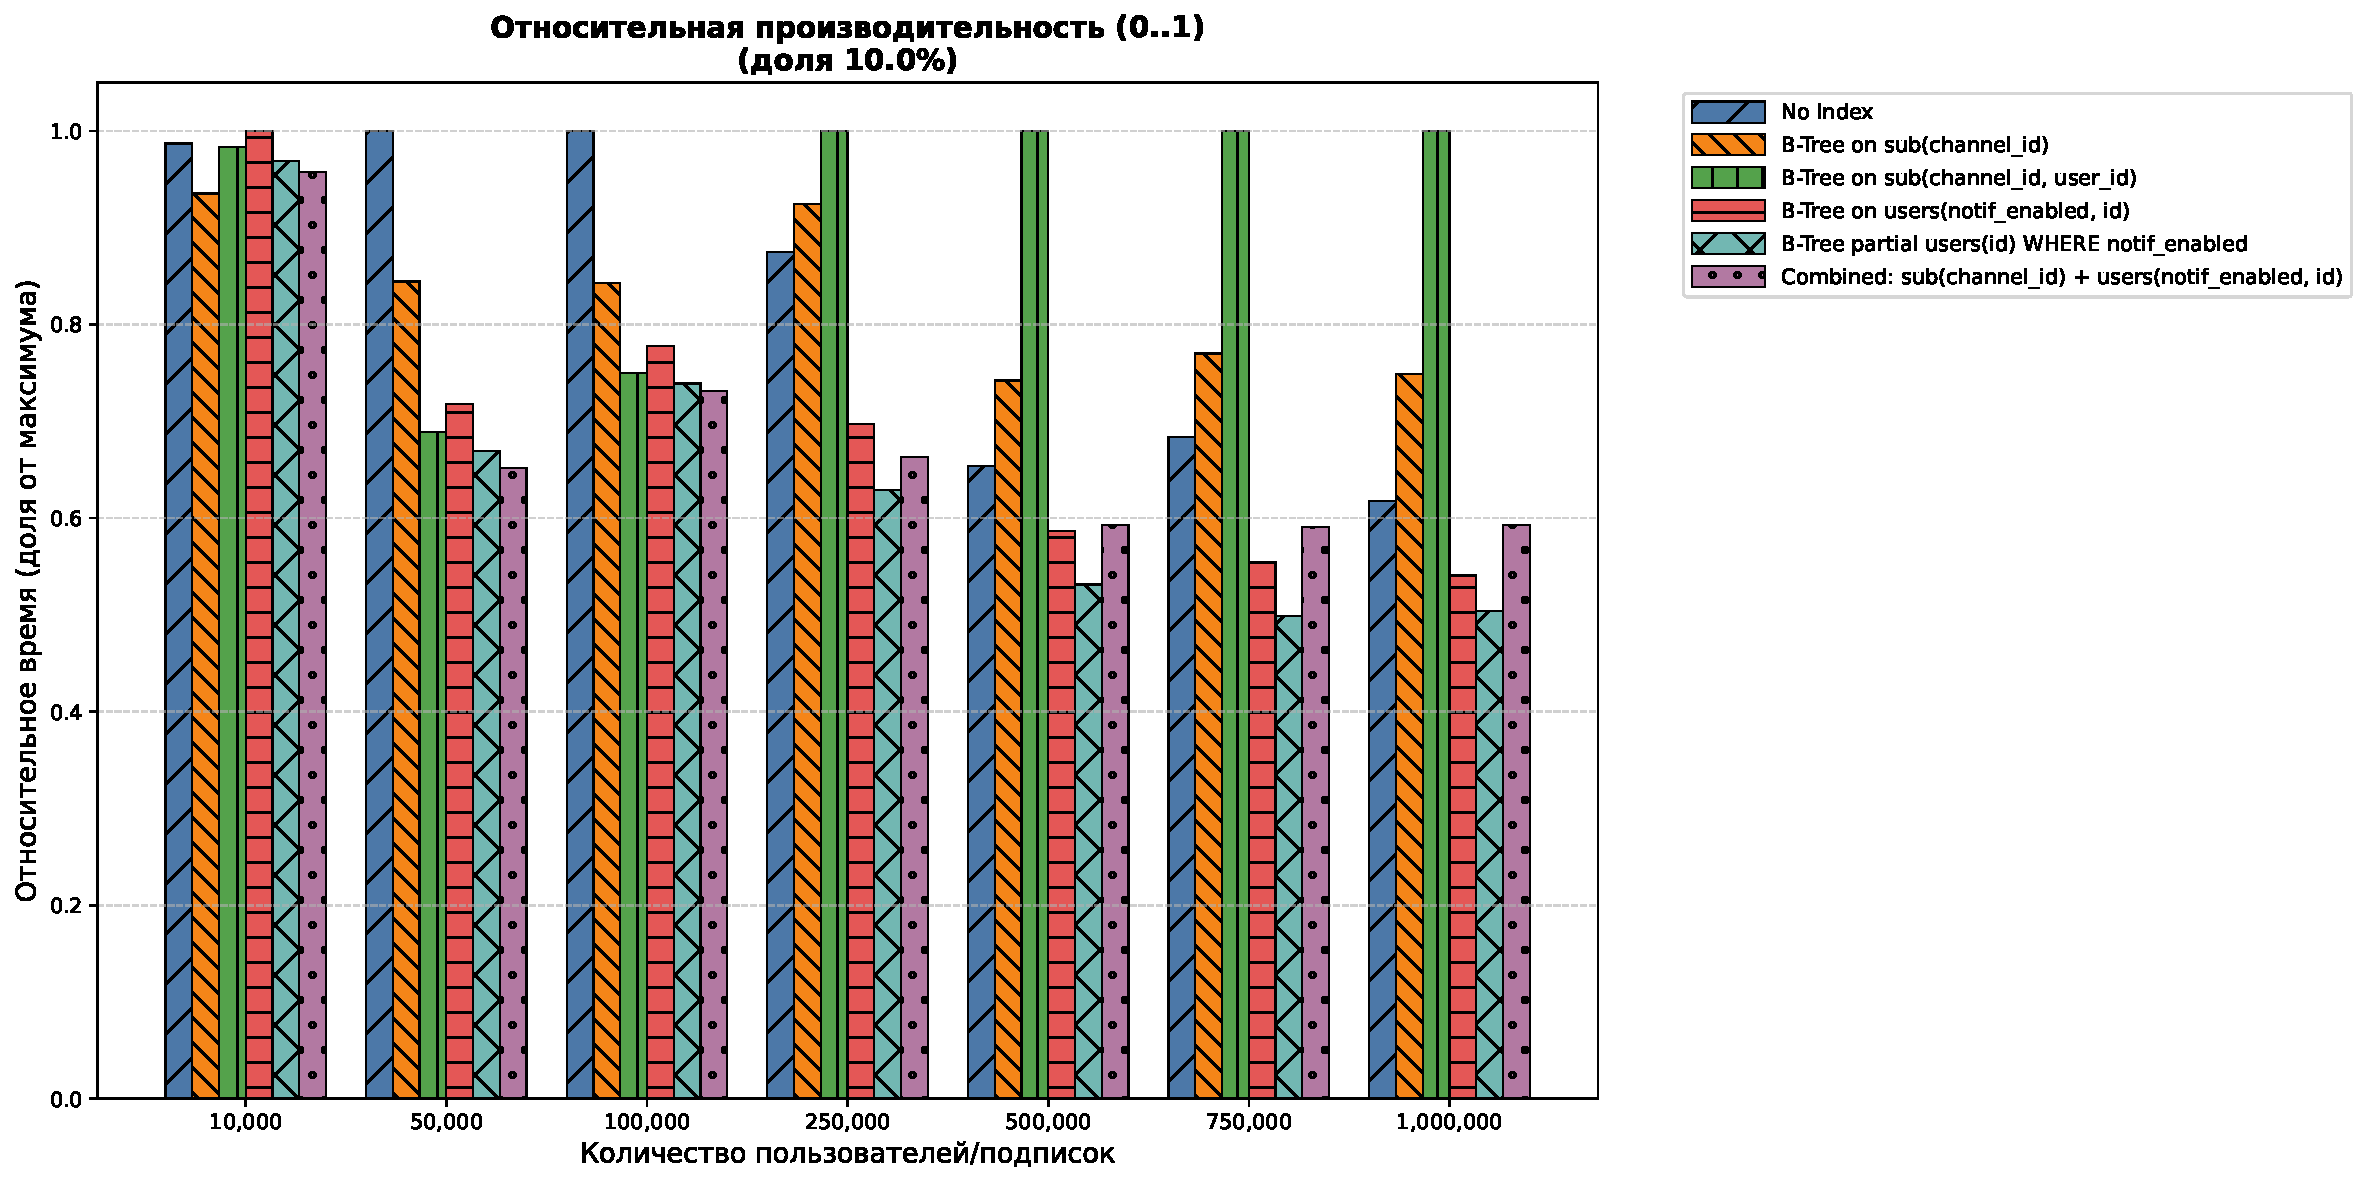
\includegraphics[width=1\linewidth]{images/benchmark_relative_0_1}
    \caption{Относительное время выполнения при доле подписчиков 10\%}
    \label{fig:benchmark-relative-0-1}
\end{figure}

По результатам исследования видно, что чем меньше строк соответствует условию, тем сильнее индекс сокращает объём чтения, и тем больше выигрыша по времени.

Для рассматриваемой процедуры ключевым фильтром является атрибут \texttt{channel\_id}.
При малой доле подписчиков условие по идентификатору канала отбирает небольшой набор строк.
Индексы \texttt{subscriptions(channel\_id)} и \texttt{subscriptions(channel\_id, user\_id)} дают заметное ускорение.
По мере роста доли подписчиков ситуация меняется: диапазон ключей для \texttt{channel\_id} становится большим, и индекс уже не даёт такого же сокращения объёма данных.

Частичный индекс \texttt{users(id)} с условием \texttt{notifications\_enabled = true} не даёт яркого эффекта при малых долях, потому что основной объём работы уже решается фильтром по \texttt{channel\_id}.
При больших долях именно фильтрация по признаку уведомлений становится существенной, и частичный индекс даёт наибольший выигрыш.


\section*{Выводы по разделу}

Таким образом, рекомендация для выбора стратегии индексирования зависит от доли подписчиков: для разреженных выборок лучше всего подходит индекс по \texttt{channel\_id}, а для плотных --- частичный индекс по признаку уведомлений.
При этом второй вариант является более универсальным, так как он обеспечивает стабильный рост производительности независимо от доли подписчиков.
\clearpage
